\section{How Arbitrary Code Execution Works}

The possibility of all arbitrary code execution is reliant on the ability to obtain access to the instruction pointer for any particular program. The instruction pointer is a processor register that points to where the current program is executing in memory. Therefore, wherever the instruction pointer is, is what’s being executed at the current time slot for that particular program. Access to the instruction pointer allows for any user to manipulate where the instruction pointer is pointing, in turn allowing for arbitrary code execution. 


In Figure 2, the instruction pointer sits between L. Address and H. Address, the address space for the currently executing program. During the instruction fetch stage of the pipelined CPU process, the instruction pointer takes the instruction at that address, and loads it into the instruction register to be used for decoding and execution. The instruction pointer then increments by an amount that varies depending on what type of instruction was fetched. For example, if the instruction was add, the instruction pointer might only increment by one. However, if the instruction was a jump command, the instruction pointer might jump further down the address space, as is evident in Figure 2. Therefore, control over the instruction pointer is paramount for arbitrary code execution to occur. (2)

\begin{figure}
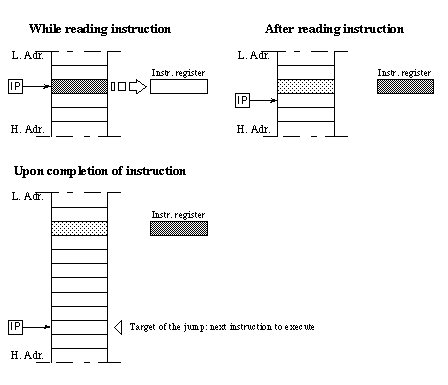
\includegraphics[width=\linewidth]{ip.png}
\caption{The process by which the instruction pointer moves.}
\end{figure}

\subsection{Buffer Overflow}

The most common way to obtain access to the instruction pointer is through buffer overflow. Buffer overflow is a simple concept made possible by flaws in programs that typically run with administrator privileges. Essentially, buffer overflow occurs when the input to a program or method in a program is larger than the developer of the program expected. As a result, the method has a way of overwriting the amount of stack memory that was allocating to it, putting the program in an unknown state. When the stack memory is overwritten, the program no longer has the capability of returning to the address that called the method. As a result, the tail end of the overwritten stack could have code that points to a different address, thus compromising the instruction pointer.


The most famous example of this is the use of strcpy in the C Standard Library. The implementation of strcpy is to copy each character until it finds a “0” in the source string, which is used to denote the end of the string. This function easily allows users to overwrite the stack memory, as referenced in Figure 3. (3)

\begin{verbatim}
#include <string.h>
#include <stdio.h> 

void foo(const char* input)
{
    char buf[10];

    printf("My stack looks like:\n%p\n%p\n%p\n%p\n%p\n% p\n\n");

    strcpy(buf, input);
    printf("%s\n", buf);

    printf("Now the stack looks like:\n%p\n%p\n%p\n%p\n%p\n%p\n\n");
}

void bar(void)
{
    printf("Augh! I've been hacked!\n");
}

int main(int argc, char* argv[])
{
    //Blatant cheating to make life easier on myself
    printf("Address of foo = %p\n", foo);
    printf("Address of bar = %p\n", bar);
    if (argc != 2) 
 {
        printf("Please supply a string as an argument!\n");
        return -1;
    } 
foo(argv[1]);
    return 0;
}
\end{verbatim}

The next figure explains how to take advantage of a compromised instruction pointer. The character array called shellcode is filled with pre-written machine code that will open a shell on the compromised system. In the main method, by manipulating the value of ret initially to be pointing to the return address of main, and then manipulating that return address to be where the contents of shellcode are stored, a user can execute the contents of shellcode.

\begin{verbatim}
char shellcode[] =
  "\xeb\x2a\x5e\x89\x76\x08\xc6\x46\x07\x00\xc7\x46\x0c\x00\x00\x00"
  "\x00\xb8\x0b\x00\x00\x00\x89\xf3\x8d\x4e\x08\x8d\x56\x0c\xcd\x80"
  "\xb8\x01\x00\x00\x00\xbb\x00\x00\x00\x00\xcd\x80\xe8\xd1\xff\xff"
  "\xff\x2f\x62\x69\x6e\x2f\x73\x68\x00\x89\xec\x5d\xc3";


void main() {
  int *ret;


  ret = (int *)&ret + 2;
  (*ret) = (int)shellcode;
}
\end{verbatim}
